\newpage
\section{Questão 12-22}

\begin{figure}[H]
	\centering
	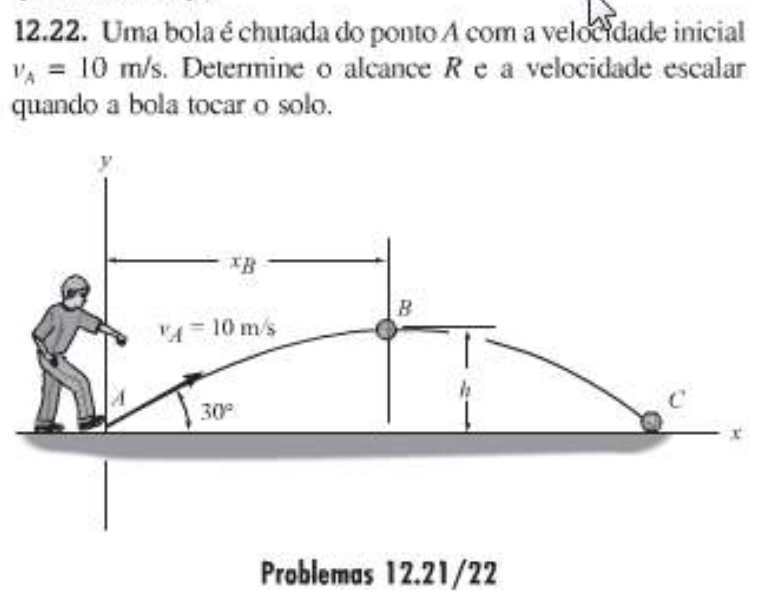
\includegraphics[width=.7\linewidth]{fundamentais/12-22.png}
	\caption{Comando da questão 12-22.}\label{fig?:12-22}
\end{figure}

Nesta questão, analisamos o movimento de um projétil lançado obliquamente com velocidade inicial \(v_A\) e ângulo de lançamento \(\alpha = 30^\circ\). Determinamos o tempo total de voo, o alcance horizontal (\(R\)) e a velocidade escalar no impacto. Também substituímos valores numéricos para ilustrar os resultados.

\subsection*{Componentes da Velocidade Inicial}
As componentes da velocidade inicial são:
\[
v_{Ax} = v_A \cos(\alpha),
\]
\[
v_{Ay} = v_A \sin(\alpha),
\]
onde:
\begin{itemize}
    \item \(v_{Ax}\): Componente horizontal da velocidade;
    \item \(v_{Ay}\): Componente vertical da velocidade.
\end{itemize}

\subsection*{Equações do Movimento}
A aceleração pode ser determinada por
\[
a(t) = \frac{dv}{dt}
\]

E a velocidade é determinada por:
\[
v(t) = \frac{ds}{dt}
\]
Manipulando as equações e combinando-as através de \(dt\), temos:

\[
a\,ds = v\,dv 
\]

Esta equação será a base das análises daqui em diante.

\subsection*{Tempo Total de Voo}

Consideramos que a aceleração horizontal \(a_x = 0\) e a vertical como \(a_y = -g\), o que permite que o alcance \(R\) seja determinado pelo tempo de voo.

O tempo total de voo ocorre quando \(y = 0\). Resolvemos a equação \(y(t) = 0\):
\[
v_{Ay} \cdot t - \frac{1}{2} g t^2 = 0.
\]

Fatorando \(t\), temos:
\[
t \left( v_{Ay} - \frac{1}{2} g t \right) = 0.
\]

A solução positiva é:
\[
t_{\text{total}} = \frac{2 v_{Ay}}{g}.
\]

\subsection*{Alcance Horizontal (\(R\))}
Substituímos \(t_{\text{total}}\) na equação do movimento horizontal para determinar o alcance:
\[
R = x(t_{\text{total}}) = v_{Ax} \cdot t_{\text{total}}.
\]

Substituindo \(t_{\text{total}} = \frac{2 v_{Ay}}{g}\):
\[
R = v_{Ax} \cdot \frac{2 v_{Ay}}{g}.
\]

Usando as expressões para \(v_{Ax}\) e \(v_{Ay}\):
\[
R = \frac{2 v_A^2 \sin(\alpha) \cos(\alpha)}{g}.
\]

Simplificando com a identidade trigonométrica \(\sin(2\alpha) = 2 \sin(\alpha) \cos(\alpha)\):
\[
R = \frac{v_A^2 \sin(2\alpha)}{g}.
\]

\subsection*{Velocidade Escalar no Impacto}
A componente horizontal da velocidade no impacto permanece constante:
\[
v_{x,\text{final}} = v_{Ax}.
\]

A componente vertical no impacto é:
\[
v_{y,\text{final}} = v_{Ay} - g \cdot t_{\text{total}}.
\]

Substituindo \(t_{\text{total}} = \frac{2 v_{Ay}}{g}\):
\[
v_{y,\text{final}} = v_{Ay} - g \cdot \frac{2 v_{Ay}}{g} = -v_{Ay}.
\]

A velocidade escalar no impacto é dada por:
\[
v_{\text{final}} = \sqrt{v_{x,\text{final}}^2 + v_{y,\text{final}}^2}.
\]

Substituindo os valores de \(v_{x,\text{final}}\) e \(v_{y,\text{final}}\):
\[
v_{\text{final}} = \sqrt{v_{Ax}^2 + (-v_{Ay})^2} = \sqrt{v_A^2}. = v_A
\]

\subsection*{Cálculos Numéricos}
Substituímos os seguintes valores:
\[
v_A = 10 \, \text{m/s}, \quad \alpha = 30^\circ = \frac{\pi}{6}, \quad g = 9.81 \, \text{m/s}^2.
\]

O alcance horizontal é:
\[
R = \frac{10^2 \sin(2 \cdot 30^\circ)}{9.81} = \frac{100 \cdot 0.866}{9.81} \approx 8.827 \, \text{m}.
\]

A velocidade escalar no impacto é:
\[
v_{\text{final}} = \sqrt{10^2} = 10 \, \text{m/s}.
\]

\subsection*{Resultados Finais}
\begin{itemize}
    \item Tempo total de voo:
    \[
    t_{\text{total}} = \frac{2 v_A \sin(\alpha)}{g}.
    \]
    \item Alcance horizontal:
    \[
    R = \frac{v_A^2 \sin(2\alpha)}{g} \approx 8.81 \, \text{m}.
    \]
    \item Velocidade escalar no impacto:
    \[
    v_{\text{final}} = v_A = 10 \, \text{m/s}.
    \]
\end{itemize}
